\section{SONARS}
The sonar sensors where already present on WTR, but the implemention lacks professionality and long term stability was at risk, both at mechanical, eletrical and software level.
The improvements are described in each of these aspects in the folling sections.

\subsection{Mechanical setup}
Instead of zipties and tape a special clamp, ball joint and housing for the HC-SR04 was designed in solidworks and 3D printed. See figure below.
There are eight sensors which are stategically placed around WTR.
The clamp (orange) is desgined to fit around the 25mm sqaure tubes which are present around WTR. 
This clamp is provided with an opening which will hold the ball clamp (red).
The ball (green) can be pressed in the ball clamp easily and will create a ball joint mechanism.
Ball is provided with a tapered shaft which is pressed into the housing (blue).
The housing holds the sonar senor, and is closed with a lid (grey).

\begin{figure}[H]
\centering
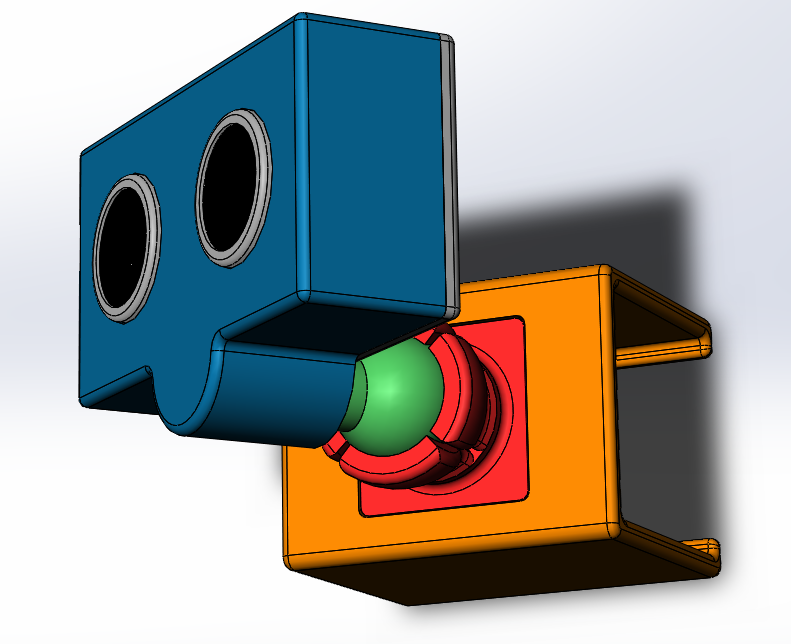
\includegraphics[width=12cm]{SonarSensorAssembly.png}
\caption{Sonar sensor assembly}
\label{fig::sonarassembly}
\end{figure}


\subsection{Electrical setup}
Instead of breadbord and a lot of lose wires a special wiring harnass was designed. 
This harnass is split into two sections, one for the three front sensors and one for the five back sensors.
The sections meet in the middle and connect to the arduino Uno.
The sections contain the common power wires, the common trigger wire and indivdual echo wires.
The wires are made from flat cable and provided with connectors which improves repair or reorientation if needed.

The wiring for the sonars can be found in the schematic below:

\begin{figure}[H]
\centering
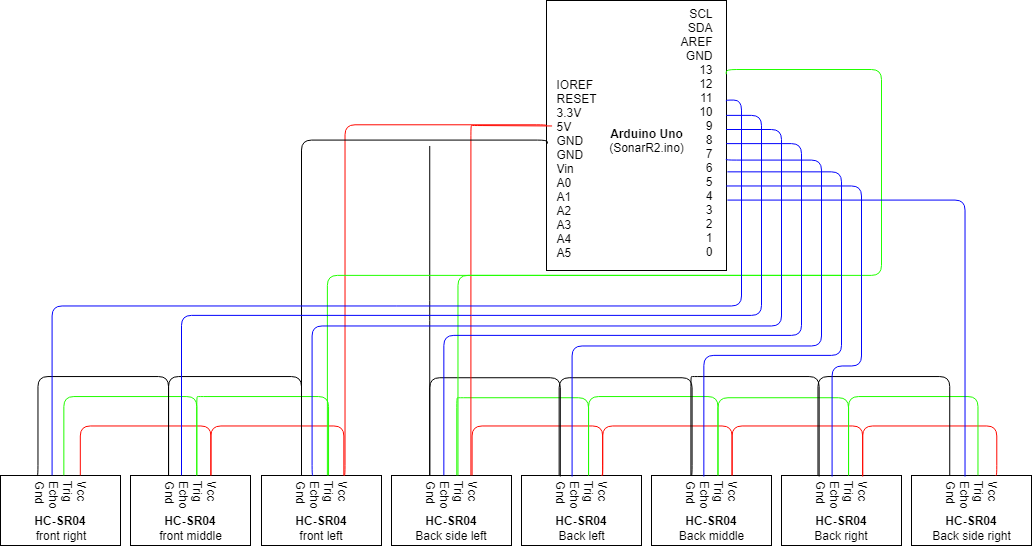
\includegraphics[width=12cm]{SonarDiagram.png}
\caption{Wiring setup for the 8 sonar sensors to Arduino communication}
\label{fig::wiringsonar}
\end{figure}

 
    